Following our preference for simplicity, we propose a three-stage architecture, shown in figure \ref{fig:architecture-stateestimation}. Measurements arriving from different sensors are first preprocessed, which, for example, includes unit conversions and coordinate transformations. In the next steps, outliers are detected. The outlier state informs the fusion of the measurements into an accurate state estimate (requirement 1), which is then used by the subsequent \gls{vdc}'s performance components and \gls{dv} software.

\begin{figure}
	\centering
	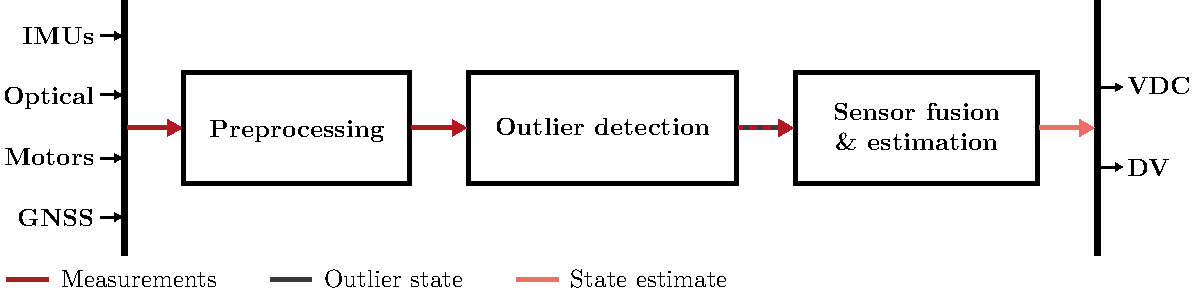
\includegraphics[width=\textwidth]{architecture_stateestimation}%
	\caption{Architecture of state estimation}
	\label{fig:architecture-stateestimation}
\end{figure}

A key feature is the unified mechanism for outlier and sensor setup detection (requirements 2 and 3). Foundation is the realization that ultimately it does not matter if a measurement is unavailable due to an invalid signal or a missing sensor, therefore both cases can be treated the same. This allows a focused effort on a single component while reducing complexity.

The following sections describe each component in detail.


\subsection{Preprocessing}
Goal of the preprocessing stage is to harmonize all measurements. Mostly, this is only a simple conversion to SI units, e.g., velocities from \si{\kilo\meter\per\hour} to \si{\meter\per\second}, or angles from \si{\deg} to \si{\radian}. Doing these conversions as early as possible simplifies subsequent computations and reduces error potential due to wrong units. For other signals, more preprocessing is necessary.

\begin{description}
\item[IMU] The most sophisticated preprocessing is required for the \glspl{imu}. The measurements are first rotated in three dimensions to correct any misalignment with the vehicle axes. Then, we need a generic \gls{imu} fusion algorithm which can take an arbitrary number of sensors with known positions and fuse them for a better estimate of the linear accelerations, yaw rate and yaw acceleration. An accurate estimate of these variables is important, because they are extensively used in the sensor fusion and performance components. This helps with reducing noise, but also enables calculation of the angular acceleration, which cannot be measured directly with our sensors. We always calculate the linear acceleration and angular velocity in three dimensions, and, in case of more than two \glspl{imu}, the angular acceleration as well. We provide two approaches for \gls{imu} fusion with the same interface, enabling drop-in replacement. Since the available \glspl{imu} need to be known at this point, performing the outlier detection here instead of the outlier detection state is necessary.

The first approach fuses measurements by averaging, and is therefore called \textit{mean-based \gls{imu} fusion}. First, the angular velocity measurements from the gyrometers are averaged. Then, the angular accelerations are derived using equation \ref{eq:angacc-from-linacc-3d} from all combinations of two \glspl{imu} and averaged. For example, in the \gls{ev}, the combinations 1--2, 2--3 and 1--3 are regarded. In case only two \glspl{imu} are available, they are assumed to have a zero $z$-position and the angular acceleration is calculated using the simplified equation \ref{eq:angacc-from-linacc-2d}. In case only a single \gls{imu} is available, we assume $\alpha = \mathbb{0}$. Finally, the linear accelerations are transformed to the \gls{cog} using equation \ref{eq:offcenter-acceleration-3d} and averaged as well, which eliminates the effect of tangential and centripetal acceleration.

The second \textit{maximum-likelihood-based \gls{imu} fusion} approach is more sophisticated and is presented in \cite{Skog.2016}, with an extension proposed in \cite{Wahlstrom.2018}. The idea is to first find a maximum-likelihood estimate for $\omega$ given the linear acceleration and angular acceleration measurements of all sensors. This is done by solving a least-squares problem using the Gauss-Newton algorithm, with a fixed number of 10 iterations instead of checking for convergence. The maximum-likelihood estimate for $a$ and $\alpha$ is then as simple as plugging the previously found estimate into a linear equation.
\end{description}

show necessary transformations for each measurement

GPS WGS84 coordinates transformed to track with first known point as reference point
maybe later mechanism to set reference point
while only speed instead of velocity is known, use as information for vx
because vy is much smaller ($\beta$ usually smaller than \SI{0.1}{\radian}) and still good enough for outlier detection

sfii transformed to \gls{cog}

\subsection{Outlier Detection}
Show diagram of AND and OR
For all EKF inputs
Plausibility check for all
For velocity, use wheels, GPS and sfii in EKF bank, different covs than in normal EKF
Plausibility for velocities rather conservative
observability and controllability
goal: support one sensor failure, more is unlikely

debouncing to increase robustness
allow manual three-way override to enable/disable sensors and override outlier detection errors

\subsection{EKF}
outlier detection sensor state and dt signal is used to create measurement mask (requirement 4)
Show input selection and state equations, jacobians
euler forward discretization
GPS is not included because it is not beneficial due to its slow response
kinematic model from~\cite[p.~156]{AlexanderWischnewski.2019}
simple without tire model: occams razor and empiric by wisch
reduces effects of noise
no heading measurements in ev, especially lack of initial heading is bad
normalize angles

prediction using differential equation
initialization
disable measurements using separate mask
input cov as process noise
